\setauthor{Arwed Schnalzenberger}

\begin{figure} [h t]
    \centering
    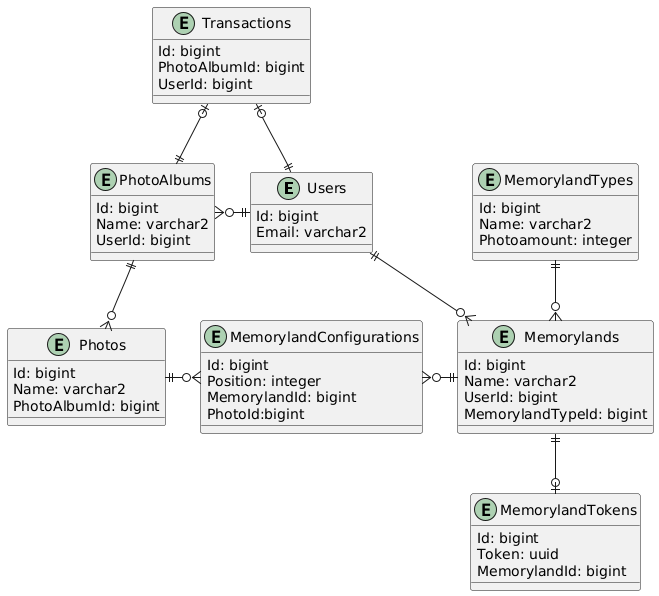
\includegraphics[scale=0.6]{puml/erd.png}
    \caption{Datenmodell}
    \label{fig:erd-diagram}
\end{figure}

Die Datenbank besteht aus insgesamt acht Tabellen, die das Backend 
für die Verwaltung von Benutzern, Fotoalben, deren Fotos und der 
Memorylands benötigt.

\section{Users}

In der Tabelle ``Users'' werden Benutzer von Memoryland gespeichert, die sich über Azure AD B2C
registriert haben. Dabei wird ein Benutzer wird mit deren Email automatisch gespeichert, sobald
er oder sie eine Aktion ausführt, die eine Speicherung im Backend erfordert. 

Der Benutzername wird nicht gespeichert, da er im Backend nicht benötigt wird und eine 
regelmäßige Aktualisierung bei Namensänderungen unnötigen Aufwand verursachen würde. Die 
E-Mail spielt in Memoryland nur als eindeutige Identifikation eines Benutzers eine Rolle.

\section{PhotoAlbums}

Diese Tabelle speichert die von Benutzern erstellten Fotoalben. Jedes Album ist eindeutig einem 
Benutzer zugeordnet, wodurch sichergestellt wird, dass ausschließlich der jeweilige Besitzer 
Zugriff darauf hat. Andere Benutzer können weder auf die Alben noch auf deren Inhalte zugreifen.

Die Alben selbst existieren als Einträge in der Datenbank, während die darin enthaltenen Fotos 
im Azure Blob Storage gespeichert werden. Das Konzept der Fotoalben wird also nur in der Datenbank 
abgebildet und hat keine direkte Entsprechung in der Speicherstruktur des Blob Storage. \footnote{\label{azure-blob-storage-note}Mehr Informationen zu ``Azure Blob Storage'' im Kapitel: \ref{subsection:azure_blob_storage_datamodel}}
Diese Struktur dient dazu, den direkten Zugriff auf den Azure Blob Storage zu minimieren und 
zu vereinfachen. Gleichzeitig ermöglicht sie dem Frontend eine sortierte und strukturierte 
Anzeige der Fotoalben.

Jeder Benutzer kann mehrere Fotoalben anlegen, wobei ein Album beliebig viele Fotos enthalten 
kann -- von keinem bis zu einer unbegrenzten Anzahl.

\section{Photos}

In dieser Tabelle werden die einzelnen Fotos mit Referenzen auf ihre jeweiligen Alben gespeichert. 
Das verwalten einzelner Fotos ist ausschließlich dem Benutzer vorbehalten, dem dieses gehört. 
Allerdings können Fotos anderen Benutzern innerhalb von Memorylands durch die Nutzung von 
SAS-Tokens angezeigt werden.

Jedes Foto gehört genau einem Album an, und innerhalb eines Albums darf kein weiteres 
Foto denselben Namen tragen. Dies gewährleistet eine eindeutige Zuordnung der Dateien für die
Benutzer.

Im Azure Blob Storage werden zur Identifikation nicht die Namen der Fotos, sondern die 
eindeutigen Identifikationsnummern verwendet. Dies ermöglicht es, dass ein Benutzer mehrere
Fotos mit identischen Namen besitzen kann, solange diese sich in unterschiedlichen Alben befinden.
\footnote{Siehe die Fußnote: \ref{azure-blob-storage-note}}

\section{Memorylands}

Ein Memoryland beinhaltet eine Sammlung von Fotos und ist immer einem bestimmten 
Memoryland-Typ zugeordnet. Der Typ eines Memorylands bestimmt unter anderem die maximale 
Anzahl an Fotos, die darin enthalten sein können.

Alle Benutzer:innen können mehrere Memorylands besitzen, die jeweils eine festgelegte Anzahl 
von Fotos an bestimmten Positionen enthalten. Die Anzahl der erlaubten Fotos pro Memoryland
hängt jeweils vom Memoryland-Typ ab.

\section{MemorylandTypes}

Diese Tabelle definiert verschiedene Typen von Memorylands. Ein Memoryland-Typ 
entspricht einer Szene in Unity und legt die maximale Anzahl an Fotos fest, die in 
einem Memoryland gespeichert werden können.

Da die Typen von den Unity-Szenen abhängen, die nur durch ein Deployment geändert werden 
können, und es keinen anderen direkten Weg gibt, festzustellen, wie viele Fotos in welcher 
Szene benötigt werden, ist es erforderlich, die Memoryland-Typen manuell in die Datenbank 
einzutragen.

\section{MemorylandConfigurations}

Diese Tabelle speichert die spezifischen Konfigurationen eines Memorylands, das heißt, 
sie definiert, welche Fotos an welchen Positionen innerhalb eines Memorylands angezeigt werden. 

Ein Memoryland kann eine beliebige Anzahl von Konfigurationen haben, wobei im Backend überprüft 
wird, ob die angegebene Position tatsächlich existiert. Zudem wird sichergestellt, dass jede 
Position innerhalb eines Memorylands nur einmal belegt wird. Es ist jedoch möglich, dass ein 
Foto in einem Memoryland mehrfach vorkommt. 

Diese Flexibilität ermöglicht es, Fotos an verschiedenen Stellen im Memoryland anzuzeigen,
ohne das die Reihenfolge der Speicherung oder anderes wichtig wäre.

\section{MemorylandTokens}

Diese Tabelle speichert die Zugriffs-Tokens eines Memorylands. Pro Memoryland kann immer nur 
ein Token gleichzeitig existieren. Benutzer:innen können mithilfe dieses Tokens auf ein 
Memoryland zugreifen und es anzeigen lassen, egal ob ihnen das Memoryland gehört oder nicht.

Die Tokens sind von der Datenbank generierte \gls{guid}s. Eine separate Tabelle für die 
Tokens wurde aus zwei wesentlichen Gründen angelegt: Zum einen ist diese Struktur eine Lösung
die eine automatische Erstellung der Tokens durch die Datenbank ermöglicht, was den 
Aufwand im Backend reduziert und eine sichere sowie eindeutige Identifikation gewährleistet. 
Zum anderen folgt die Trennung der Tokens in eine eigene Tabelle dem Prinzip der 
``Separation of Concerns''.

``\emph{Separation of Concerns}'' ist ein Prinzip der Softwareentwicklung, bei dem 
verschiedene Aspekte eines Systems oder einer Anwendung klar voneinander getrennt werden. 
In diesem Fall enthält die Tabelle der Memorylands allgemeine Informationen über die 
erstellten Memorylands, während die Tabelle der Tokens die separate Verantwortung 
für die Tokens übernimmt. Durch diese Trennung ist es einfacher neue Sicherheitsmechanismen 
oder Berechtigungsstufen oder anderes hinzuzufügen oder zu entfernen.
\footnote{Alle Informationen zu ``Separation of Concerns'' stammen von: \cite{kulkarni2003separation}}

\section{Transactions}

Diese Tabelle dient der Verwaltung von Transaktionen, die verwendet werden, um das Hochladen 
großer Fotoalben effizienter zu gestalten. Besonders bei umfangreichen Bildersammlungen, 
wie sie beispielsweise nach einer Reise oder einem Event anfallen, kann der Upload-Prozess 
durch verschiedene Faktoren unterbrochen werden -- sei es durch eine instabile 
Internetverbindung, einen Verbindungsabbruch oder anderem. Um zu verhindern, dass 
Benutzer:innen in solchen Fällen den gesamten Upload erneut starten müssen, wird ein 
Mechanismus für „Resumable Uploads“ verwendet.

In dieser Diplomarbeit werden solche Upload-Vorgänge synonym als „Transaktionen“ und 
„Resumable Uploads“ bezeichnet. Jede:r Benutzer:in kann zu einem bestimmten Zeitpunkt 
genau eine aktive Transaktion haben. In der Tabelle wird außerdem eine Referenz auf 
das jeweilige Fotoalbum gespeichert, in das die Bilder hochgeladen werden. 
Dies ermöglicht es, einen begonnenen Upload gezielt einem bestimmten Album zuzuordnen 
und den Prozess genau dort fortzusetzen, wo er unterbrochen wurde, was Benutzer:innen
dabei helfen kann, sich daran zu erinnern, wofür der Upload gedacht war.

\subsection{Probleme bei der Implementierung}
\label{subsection:implementation-problems-resumable-upload}

Ursprünglich war vorgesehen, zusätzlich den lokalen Dateipfad der hochgeladenen 
Dateien in der Datenbank zu speichern. Dieses Feature konnte jedoch aufgrund von 
Sicherheitsrichtlinien nicht umgesetzt werden, da das Speichern vollständiger 
Dateipfade potenzielle Risiken im Hinblick auf Datenschutz und Zugriffsbeschränkungen 
mit sich gebracht hätte.

Für den Upload ganzer Fotoalben wurde die HTML5-Funktion \emph{webkitdirectory} genutzt, 
die es ermöglicht, komplette Verzeichnisse auszuwählen und deren Inhalte hochzuladen. 
Allerdings erlaubt \emph{webkitdirectory} aus Sicherheitsgründen keinen Zugriff auf absolute 
Dateipfade. Stattdessen werden nur relative Pfade bereitgestellt, wodurch die 
ursprüngliche Idee, vollständige Dateipfade in der Datenbank zu speichern, technisch 
nicht umsetzbar war. \footnote{Alle Informationen zu dem ``webkitdirectory'' stammen von: \cite{MozillaFoundation}}

